\section{Dataset and Cleaning}
\label{sec:dataset}

\begin{figure*}[t]
  \centering
  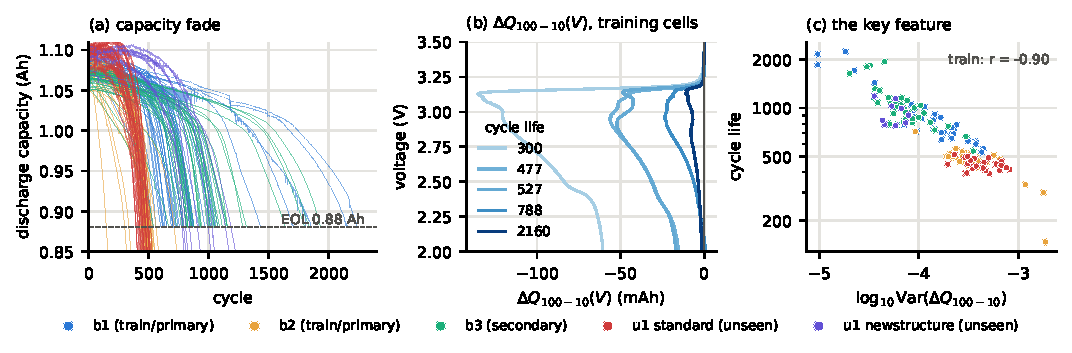
\includegraphics[width=\textwidth]{fig_data}
  \caption{(a) Discharge capacity of all 163 cells. (b) $\dq$ of five
  training cells spanning the life range. (c) Log variance of $\dq$ against
  cycle life for all cells.}
  \label{fig:data}
\end{figure*}

\subsection{Batches and test procedures}
We use the public dataset of~\cite{severson2019,matr_data}: three batches
of the original study (b1--b3, 124 cells, 69 distinct fast-charging policies with
0--80\,\% charge times of 9--13\,min) and a fourth batch from the same
repository, u1 (2018-02-20), which the original study did not use. We keep
the paper's split: 41 training and 43 primary-test cells from b1 and b2, and
the 40 cells of b3 as the secondary test set. u1 has 39 cells with a cycle
life: 30 \emph{standard} cells and 9 marked \texttt{-newstructure}, all
charging to 80\,\% in 10\,min. Its 8 other cells change policy during the
test or were stopped early and have no life label.

Only the fast charge differs between cells, but the rest of the procedure
differs between batches (Table~\ref{tab:batches}), which we measured from
the raw current traces at cycle 50. b3 was also tested about a year after
b1 and b2, so its cells start with less capacity~\cite{severson2019}.

\begin{table}[!htb]
\centering
\caption{Test procedure of each set, measured at cycle 50. Rests: pauses
per cycle; CV end: how the 3.6\,V hold ends; $Q_2$: median capacity at
cycle 2 (Ah); $t_c$: median cycle duration (min).}
\label{tab:batches}
\small
\setlength{\tabcolsep}{3.5pt}
\begin{tabular}{@{}lrccccc@{}}
\toprule
Set & $n$ & Life & Rests & CV end & $Q_2$ & $t_c$ \\
\midrule
b1 & 41 & 534--2237 & 1\,min & time limit & 1.078 & 52 \\
b2 & 43 & 148--713 & 2$\times$5\,min & time limit & 1.072 & 60 \\
b3 & 40 & 541--1935 & 4$\times$5\,s & C/20 & 1.065 & 46 \\
u1 std & 30 & 392--514 & 2$\times$5\,min & C/50 & 1.096 & 69 \\
u1 new & 9 & 777--1186 & 2$\times$10\,s & C/20 & 1.091 & 48 \\
\bottomrule
\end{tabular}
\end{table}

\subsection{Cleaning}
We first apply the cleaning of the authors' code: five b1 cells that never
reached end of life and six faulty b3 channels are dropped, and five b1 cells
that continued in b2 are joined. All 124 cells then match the paper's
Supplementary Table~9 in split, batch and cycle life. Inspecting every batch
showed further faults, fixed by the rules in Table~\ref{tab:cleaning}. Bad
values are set to NaN, never overwritten or invented. Rules C1--C4 affect
0.06\,\% of capacity values and 3.7\,\% of resistance values in cycles
2--100 (the latter almost all from six u1 cells with no resistance record).

\begin{table}[!htb]
\centering
\caption{Cleaning rules added to those of~\cite{severson2019}.}
\label{tab:cleaning}
\small
\setlength{\tabcolsep}{2.5pt}
\begin{tabular}{@{}l>{\raggedright\arraybackslash}p{0.43\columnwidth}>{\raggedright\arraybackslash}p{0.47\columnwidth}@{}}
\toprule
& Fault & Rule \\
\midrule
C1 & Empty first record (b1); resistance $=0$ & set to NaN \\
C2 & Capacity spikes/dips (e.g.\ 2.88\,Ah), test-wide pauses in b2, u1 & $>20$\,mAh from 5-cycle median $\to$ NaN \\
C3 & Corrupt $Q(V)$ curve at glitch cycles & use nearest valid cycle ($\pm2$) \\
C4 & Charge time stuck at 20\,min & set to NaN \\
C5 & Temperature probe off the cell (4 cells) & flag; excluded from F3 \\
C6 & Resistance logger stuck (b1c18, cycles 2--53) & $\ge5$ equal values $\to$ NaN \\
C7 & Time-stamp gaps of hours to days & left out of $\int T\,dt$ \\
\bottomrule
\end{tabular}
\end{table}

\subsection{Exploratory observations}
\label{sec:eda}
\begin{enumerate}
  \item Capacity is nearly flat, or even rises, for most of life and then
  falls at a knee (Fig.~\ref{fig:data}a); lives range from 148 to 2237
  cycles.
  \item $\dq$ is negative mainly on the 3.0--3.2\,V plateau, and its
  magnitude grows with shorter life (Fig.~\ref{fig:data}b). Its log
  variance alone gives $r=-0.90$ with log life on the training cells
  (Fig.~\ref{fig:data}c).
  \item The batches overlap only partly. b2 and u1-standard cells mostly live
  400--550 cycles, b1 and b3 cells much longer. Within u1 the correlation
  is weak ($r=-0.38$ standard, $-0.27$ \texttt{newstructure}), so much of
  the overall trend separates batches and procedures.
  \item Several F3 features mainly encode the procedure. The temperature
  integral tracks cycle duration ($r=0.92$), which is set by the rests
  (Table~\ref{tab:batches}), and the mean charge time varies only within b1.
\end{enumerate}
